\chapter{Verwantschap lezen: fylogenetische bomen}\label{ch:g12:phylogenetic-trees}

In 1837 schetste Darwin op een bladzijde van een privéschrift een
vertakkende lijn met enkele twijgen en schreef er twee woorden boven: "I
think". Die schets stelde voor dat \omterm{def:g10:biodiversity-scales:species}{soorten} met elkaar verwant zijn zoals
de twijgen van een boom --- door afstamming uit gemeenschappelijke takken
--- en dat hun verwantschap te reconstrueren valt. Vandaag is de schets
een gewoon gereedschap: een \omterm{def:g12:phylogenetic-trees:tree}{fylogenetische boom}, gebouwd uit gedeelde
kenmerken en uit \omterm{def:g10:universal-dna:information}{DNA}, en volgens regels gelezen. Dit hoofdstuk leert die
regels: hoe je uit een kenmerkentabel een boom bouwt, hoe je er een leest
zonder haar verkeerd te lezen, en hoe moleculen haar in een klok
veranderen.

\section{Wat een boom zegt}

\begin{definition}[Fylogenetische boom]\label{def:g12:phylogenetic-trees:tree}
Een \emph{fylogenetische boom}\index{fylogenetische boom} is een schema
van de verwantschap van een aantal \omterm{def:g10:biodiversity-scales:species}{soorten} (of andere groepen). Haar
toppen zijn de vergeleken \omterm{def:g10:biodiversity-scales:species}{soorten}; elke \emph{knoop} waar twee takken
samenkomen staat voor hun jongste gemeenschappelijke voorouder --- een
verondersteld \omterm{def:g12:selection-drift-speciation:population}{populatie}, geen bekend fossiel; de \emph{wortel} is de
gemeenschappelijke voorouder van alle. Twee \omterm{def:g10:biodiversity-scales:species}{soorten} zijn nauwer verwant
dan een derde wanneer hun gemeenschappelijke voorouder (hun knoop) jonger
is dan de knoop die zij met de derde delen. Verwantschap wordt uit de
knopen afgelezen, en nooit uit de plaats van de toppen van links naar
rechts.
\end{definition}

\begin{proposition}[Regels voor het lezen]\label{prop:g12:phylogenetic-trees:rules}
\begin{itemize}
  \item Een boom mag bij elke knoop worden gedraaid zonder dat haar
        betekenis verandert: de volgorde van de toppen is willekeurig.
  \item Een knoop heeft geen naam en is geen van de toppen: een \omterm{def:g10:biodiversity-scales:species}{soort} is
        op de boom nooit de voorouder van een andere \omterm{def:g10:biodiversity-scales:species}{soort}; twee toppen
        zijn \emph{zustergroepen}, afstammend van een gedeelde voorouder.
  \item Een groep die uit een voorouder en \emph{al} haar nakomelingen
        bestaat --- alles voorbij één knoop --- is een
        \emph{clade}\index{clade}, de enige \omterm{def:g10:biodiversity-scales:species}{soort} groep die een
        fylogenetische indeling een naam geeft.
  \item Taklengtes dragen alleen informatie als de boom dat zegt (tijd,
        of aantal veranderingen); anders telt alleen de volgorde van de
        vertakkingen.
\end{itemize}
\end{proposition}
\admitted

\begin{omfigure}
\begin{tikzpicture}[font=\small, line cap=round]
  % tree 1
  \begin{scope}
    \draw[thick] (0,0) -- (1,0);
    \draw[thick] (1,0) -- (1,1.2) -- (4.5,1.2);
    \draw[thick] (1,0) -- (1,-1.2) -- (2.2,-1.2);
    \draw[thick] (2.2,-1.2) -- (2.2,-0.5) -- (4.5,-0.5);
    \draw[thick] (2.2,-1.2) -- (2.2,-1.9) -- (3.4,-1.9);
    \draw[thick] (3.4,-1.9) -- (3.4,-1.5) -- (4.5,-1.5);
    \draw[thick] (3.4,-1.9) -- (3.4,-2.3) -- (4.5,-2.3);
    \node[anchor=west] at (4.6,1.2) {kikker}; \node[anchor=west] at (4.6,-0.5) {hagedis};
    \node[anchor=west] at (4.6,-1.5) {muis}; \node[anchor=west] at (4.6,-2.3) {mens};
    \fill[omThm] (1,0) circle (2pt); \fill[omThm] (2.2,-1.2) circle (2pt); \fill[omThm] (3.4,-1.9) circle (2pt);
    \node[anchor=north, align=center] at (2.8,-2.7) {boom A};
  \end{scope}
  % tree 2: same topology, rotated
  \begin{scope}[xshift=8cm]
    \draw[thick] (0,0) -- (1,0);
    \draw[thick] (1,0) -- (1,1.2) -- (2.2,1.2);
    \draw[thick] (2.2,1.2) -- (2.2,1.9) -- (3.4,1.9);
    \draw[thick] (3.4,1.9) -- (3.4,2.3) -- (4.5,2.3);
    \draw[thick] (3.4,1.9) -- (3.4,1.5) -- (4.5,1.5);
    \draw[thick] (2.2,1.2) -- (2.2,0.5) -- (4.5,0.5);
    \draw[thick] (1,0) -- (1,-1.2) -- (4.5,-1.2);
    \node[anchor=west] at (4.6,2.3) {mens}; \node[anchor=west] at (4.6,1.5) {muis};
    \node[anchor=west] at (4.6,0.5) {hagedis}; \node[anchor=west] at (4.6,-1.2) {kikker};
    \fill[omThm] (1,0) circle (2pt); \fill[omThm] (2.2,1.2) circle (2pt); \fill[omThm] (3.4,1.9) circle (2pt);
    \node[anchor=north, align=center] at (2.8,-2.7) {boom B: dezelfde boom};
  \end{scope}
\end{tikzpicture}

{\small Twee tekeningen van één boom. De takken bij elke knoop draaien
verandert de volgorde van de toppen, maar geen enkele verwantschap: in
beide zijn muis en mens zusters, is de hagedis hun naaste verwant en staat
de kikker het verst weg. "De hagedis staat tussen de kikker en de muis in"
uit boom A lezen zou een vergissing zijn.}
\end{omfigure}

\begin{example}[Verkeerde lezingen om te vermijden]\label{ex:g12:phylogenetic-trees:misreadings}
"Mensen stammen af van chimpansees": nee --- op de boom zijn mensen en
chimpansees zustertoppen, afstammend van een gemeenschappelijke voorouder
die geen van beide was. "De kikker is primitiever": nee --- elke top is
een hedendaagse \omterm{def:g10:biodiversity-scales:species}{soort} met evenveel geschiedenis sinds de wortel; de
kikkerlijn is even lang geëvolueerd als de onze. "De hagedis staat dichter
bij de kikker dan bij de muis" (uit boom A): nee --- hagedis en muis delen
een jongere knoop.
\end{example}

\section{Een boom bouwen uit kenmerken}

\begin{definition}[Voorouderlijke en afgeleide toestanden]\label{def:g12:phylogenetic-trees:states}
Een \emph{kenmerk} is een eigenschap die tussen de vergeleken \omterm{def:g10:biodiversity-scales:species}{soorten}
verschilt (de aanwezigheid van een wervelkolom, van vier ledematen, van
een amnionei, van haar). Elk kenmerk heeft een \emph{voorouderlijke}
toestand --- die welke de gemeenschappelijke voorouder van de groep had
--- en één of meer \emph{afgeleide} toestanden die later in een bepaalde
lijn verschenen. Alleen \emph{gedeelde afgeleide toestanden} wijzen op
verwantschap: twee \omterm{def:g10:biodiversity-scales:species}{soorten} die een afgeleide toestand delen, hebben die
geërfd van de voorouder waarbij zij ontstond. Een gedeelde voorouderlijke
toestand zegt niets, want ieders voorouder had haar.
\end{definition}

\begin{method}[Van een kenmerkentabel tot een boom]\label{met:g12:phylogenetic-trees:build}
\begin{enumerate}
  \item Maak een tabel: \omterm{def:g10:biodiversity-scales:species}{soorten} in de rijen, kenmerken in de kolommen, 1
        voor de afgeleide toestand en 0 voor de voorouderlijke. Bepaal
        welke toestand voorouderlijk is door te vergelijken met een
        \emph{buitengroep}, een \omterm{def:g10:biodiversity-scales:species}{soort} waarvan bekend is dat zij buiten de
        bestudeerde groep valt.
  \item Zoek de afgeleide toestand die door de meeste \omterm{def:g10:biodiversity-scales:species}{soorten} wordt
        gedeeld: die bepaalt de eerste, grootste \omterm{prop:g12:phylogenetic-trees:rules}{clade}. Zoek daarbinnen
        de volgende afgeleide toestand die door de meeste \omterm{def:g10:biodiversity-scales:species}{soorten} wordt
        gedeeld, enzovoort.
  \item Teken de in elkaar geschoven \omterm{prop:g12:phylogenetic-trees:rules}{clades} als een boom: elke gedeelde
        afgeleide toestand markeert één knoop, en het kenmerk wordt
        geschreven op de tak waar het verscheen.
  \item Kijk naar tegenspraken: een kenmerk dat wordt gedeeld door
        \omterm{def:g10:biodiversity-scales:species}{soorten} die andere kenmerken uit elkaar plaatsen, is ofwel twee
        keer ontstaan (convergentie) ofwel één keer verloren gegaan. Kies
        de boom die in het geheel de minste veranderingen vergt --- de
        meest \emph{spaarzame} boom.
\end{enumerate}
\end{method}

\begin{omfigure}
\begin{tikzpicture}[font=\small, line cap=round]
  % matrix
  \node[anchor=east] at (-0.2,2.4) {};
  \matrix (m) [matrix of nodes, nodes={font=\small, minimum width=1.1cm, minimum height=0.5cm, anchor=center},
               column 1/.style={nodes={anchor=east, minimum width=1.6cm}}] at (1.6,0.5) {
    \phantom{o} & kaken & ledematen & amnion & haar \\
    prik & 0 & 0 & 0 & 0 \\
    forel & 1 & 0 & 0 & 0 \\
    kikker & 1 & 1 & 0 & 0 \\
    hagedis & 1 & 1 & 1 & 0 \\
    muis & 1 & 1 & 1 & 1 \\
  };
  \draw (m-1-1.south west) -- (m-1-5.south east);
  \draw (m-1-2.north west) -- (m-6-2.south west);
  % tree
  \begin{scope}[xshift=7.2cm, yshift=-1.4cm]
    \draw[thick] (0,0) -- (0.8,0);
    \draw[thick] (0.8,0) -- (0.8,3.2) -- (5,3.2);
    \draw[thick] (0.8,0) -- (0.8,-0.6) -- (1.8,-0.6);
    \draw[thick] (1.8,-0.6) -- (1.8,2.4) -- (5,2.4);
    \draw[thick] (1.8,-0.6) -- (1.8,-1.0) -- (2.8,-1.0);
    \draw[thick] (2.8,-1.0) -- (2.8,1.6) -- (5,1.6);
    \draw[thick] (2.8,-1.0) -- (2.8,-1.3) -- (3.8,-1.3);
    \draw[thick] (3.8,-1.3) -- (3.8,0.8) -- (5,0.8);
    \draw[thick] (3.8,-1.3) -- (3.8,-1.5) -- (5,-1.5);
    \node[anchor=west] at (5.1,3.2) {prik}; \node[anchor=west] at (5.1,2.4) {forel};
    \node[anchor=west] at (5.1,1.6) {kikker}; \node[anchor=west] at (5.1,0.8) {hagedis};
    \node[anchor=west] at (5.1,-1.5) {muis};
    \foreach \x/\y/\t in {1.3/-0.6/kaken, 2.3/-1.0/ledematen, 3.3/-1.3/amnion, 4.4/-1.5/haar}
      { \draw[very thick, omThm] (\x,\y+0.15) -- (\x,\y-0.15); \node[font=\scriptsize, omThm, anchor=north] at (\x,\y-0.2) {\t}; }
    \node[anchor=east, font=\scriptsize] at (-0.1,0) {buitengroep: prik};
  \end{scope}
\end{tikzpicture}

{\small Van tabel naar boom. Elke afgeleide toestand (1) die door een
groep \omterm{def:g10:biodiversity-scales:species}{soorten} wordt gedeeld, markeert de knoop van hun gemeenschappelijke
voorouder; de rode streepjes geven aan waar elk kenmerk verscheen. De
prik, die elke afgeleide toestand mist, is de buitengroep die de
voorouderlijke toestanden vastlegt.}
\end{omfigure}

\begin{example}[Een tegenspraak opgelost door spaarzaamheid]\label{ex:g12:phylogenetic-trees:parsimony}
Voeg "vleugels" toe aan een tabel met vleermuis, duif en muis. Vleugels
zouden de vleermuis bij de duif groeperen; haar en melk groeperen de
vleermuis bij de muis. Een boom met vleermuis en muis samen vergt dat
vleugels twee keer zijn ontstaan (twee veranderingen); een boom met
vleermuis en duif samen vergt dat haar, melk, de zoogdierkaak en een
tiental andere kenmerken elk twee keer zijn ontstaan. De eerste boom is
veel spaarzamer: de vleugels zijn een convergentie, de zoogdierkenmerken
een gemeenschappelijke erfenis. Spaarzaamheid bewijst de boom niet; zij
kiest de minst onwaarschijnlijke.
\end{example}

\section{Bomen uit moleculen}

\begin{proposition}[Moleculaire fylogenie]\label{prop:g12:phylogenetic-trees:molecular}
Een \omterm{def:g10:universal-dna:gene}{gen} of \omterm{def:g11:gene-expression:protein}{eiwit} dat alle vergeleken \omterm{def:g10:biodiversity-scales:species}{soorten} delen, is op zichzelf al een
kenmerkentabel: elke plaats in de volgorde is een kenmerk, en elke
\omterm{def:g10:universal-dna:nucleotide}{nucleotide} of elk \omterm{def:g10:chemistry-of-life:families}{aminozuur} een toestand. De volgordes naast elkaar
leggen en de verschillen tussen elk paar tellen levert een
afstandenmatrix op, waaruit een boom wordt gebouwd door de dichtstbijzijnde
paren als eerste samen te voegen. De moleculaire boom, berekend uit
volgordes die niets aan de anatomie te danken hebben, komt in de grote
meerderheid van de gevallen met de anatomische boom overeen --- de
sterkste toets van beide.
\end{proposition}
\begin{proof}[Bewijsmateriaal]
\cref{ch:g10:common-ancestry} gaf de afstanden van cytochroom c bij de
\omterm{def:g10:common-ancestry:bodyplan}{gewervelden}, die de kaders van hun skeletten weer opleveren. Bij de
primaten zijn de volgordes van tientallen \omterm{def:g10:universal-dna:gene}{genen} het eens: mens en
chimpansee verschillen ongeveer 1.2\% in hun \omterm{def:g10:universal-dna:information}{DNA}, elk van beide 1.6\% van
de gorilla, de drie 3\% van de orang-oetan, en de mensapen 7\% van de
makaak. Een boom die uit welk van die \omterm{def:g10:universal-dna:gene}{genen} dan ook wordt gebouwd, heeft
dezelfde vorm; de weinige uitzonderingen betreffen de jongste knopen,
waar de verschillen het kleinst zijn.
\end{proof}

\begin{omfigure}
\begin{tikzpicture}[font=\small, line cap=round]
  \draw[thick] (0,0) -- (1,0);
  \draw[thick] (1,0) -- (1,2.4) -- (8,2.4);
  \draw[thick] (1,0) -- (1,-0.8) -- (3,-0.8);
  \draw[thick] (3,-0.8) -- (3,1.2) -- (8,1.2);
  \draw[thick] (3,-0.8) -- (3,-1.4) -- (5.2,-1.4);
  \draw[thick] (5.2,-1.4) -- (5.2,0) -- (8,0);
  \draw[thick] (5.2,-1.4) -- (5.2,-2.0) -- (6.4,-2.0);
  \draw[thick] (6.4,-2.0) -- (6.4,-1.2) -- (8,-1.2);
  \draw[thick] (6.4,-2.0) -- (6.4,-2.8) -- (8,-2.8);
  \node[anchor=west] at (8.1,2.4) {makaak}; \node[anchor=west] at (8.1,1.2) {orang-oetan};
  \node[anchor=west] at (8.1,0) {gorilla}; \node[anchor=west] at (8.1,-1.2) {chimpansee};
  \node[anchor=west] at (8.1,-2.8) {mens};
  \foreach \x/\t in {1/{25}, 3/{14}, 5.2/{9}, 6.4/{6}}
    { \fill[omThm] (\x,-3.4) circle (0); \node[font=\scriptsize, omThm, anchor=north] at (\x,-3.4) {\t}; \draw[gray, dashed] (\x,-3.3) -- (\x,-3.0); }
  \draw[->, gray] (0.5,-3.5) -- (8,-3.5) node[midway, below=7pt, font=\scriptsize] {miljoenen jaren geleden (knopen gedateerd met de moleculaire klok en fossielen)};
  \node[font=\scriptsize, anchor=south] at (7.2,-1.05) {1.2\% van het DNA};
  \node[font=\scriptsize, anchor=south] at (6.6,0.15) {1.6\%};
  \node[font=\scriptsize, anchor=south] at (5.5,1.35) {3\%};
  \node[font=\scriptsize, anchor=south] at (4.5,2.55) {7\% van het DNA verschilt};
\end{tikzpicture}

{\small De boom van vijf primaten uit een DNA-vergelijking. Mens en
chimpansee zijn zustergroepen; daarna sluit de gorilla zich bij hen aan,
dan de orang-oetan, dan de makaak. Het percentage op elke tak is het
verschil in \omterm{def:g10:universal-dna:information}{DNA} tussen de \omterm{def:g10:biodiversity-scales:species}{soorten} die zij verbindt; de dateringen eronder
komen van de moleculaire klok, met fossielen geijkt.}
\end{omfigure}

\begin{proposition}[De moleculaire klok]\label{prop:g12:phylogenetic-trees:clock}
Voor een gegeven \omterm{def:g10:universal-dna:gene}{gen} hopen de verschillen tussen twee lijnen zich over
lange perioden met een ruwweg constant tempo op, omdat de meeste
substituties neutraal zijn en door drift worden vastgelegd met het tempo
waarin zij ontstaan. Het aantal verschillen tussen twee \omterm{def:g10:biodiversity-scales:species}{soorten} is dus
evenredig met de tijd sinds hun gemeenschappelijke voorouder. Op één knoop
geijkt die door fossielen is gedateerd, dateert de klok de andere --- met
het voorbehoud dat de tempo's tussen \omterm{def:g10:universal-dna:gene}{genen} en tussen lijnen verschillen,
en dat de ijking haar eigen onzekerheid meebrengt.
\end{proposition}
\admitted

\begin{omfigure}
\begin{tikzpicture}
\begin{axis}[
  width=0.84\linewidth, height=5.6cm,
  axis x line=bottom, axis y line=left,
  xmin=0, xmax=30, ymin=0, ymax=8,
  xlabel={tijd sinds de gemeenschappelijke voorouder (miljoen jaar, uit fossielen)},
  ylabel={verschil in DNA (\%)},
  xlabel style={font=\small, at={(axis description cs:0.5,-0.12)}, anchor=north},
  ylabel style={font=\small},
  tick label style={font=\small}, xtick={0,5,10,15,20,25,30}, ytick={0,2,4,6,8},
  clip=false,
]
\addplot[only marks, mark=*, mark size=2pt, omThm] coordinates {(6,1.2) (9,1.6) (14,3.0) (25,7.0)};
\addplot[thick, omDef, domain=0:28] {0.27*x};
\node[font=\scriptsize, anchor=west] at (axis cs:6.4,1.0) {mens--chimpansee};
\node[font=\scriptsize, anchor=west] at (axis cs:9.4,1.5) {--gorilla};
\node[font=\scriptsize, anchor=west] at (axis cs:14.4,2.9) {--orang-oetan};
\node[font=\scriptsize, anchor=east] at (axis cs:24.6,7.1) {--makaak};
\end{axis}
\end{tikzpicture}

{\small De moleculaire klok bij de primaten: het verschil in \omterm{def:g10:universal-dna:information}{DNA} tegen de
ouderdom van de gemeenschappelijke voorouder. De punten liggen dicht bij
een rechte lijn van ongeveer 0.27\% per miljoen jaar; met die lijn kan een
knoop zonder fossielen uit zijn DNA-verschil worden gedateerd.}
\end{omfigure}

\begin{example}[Een knoop dateren]\label{ex:g12:phylogenetic-trees:dating}
Twee \omterm{def:g10:biodiversity-scales:species}{soorten} verschillen 4.5\% in hun \omterm{def:g10:universal-dna:information}{DNA}; bij 0.27\% per miljoen jaar
leefde hun gemeenschappelijke voorouder zo'n 17 miljoen jaar geleden. Die
schatting veronderstelt dat het tempo van de primaten geldt; voor een \omterm{def:g10:universal-dna:gene}{gen}
dat twee keer zo snel evolueert, of in een lijn met kortere generaties,
zou diezelfde 4.5\% de helft van die tijd betekenen. Een klok is niet
beter dan haar ijking.
\end{example}

\section{Indelen, vanuit bomen}

\begin{proposition}[Indelen naar afstamming]\label{prop:g12:phylogenetic-trees:classification}
Een fylogenetische indeling geeft alleen \omterm{prop:g12:phylogenetic-trees:rules}{clades} een naam: groepen die door
een knoop worden bepaald en al haar nakomelingen bevatten. Vertrouwde
groepen die die toets niet doorstaan, worden niet gebruikt: "vissen"
sluit de viervoeters uit die van dezelfde knoop afstammen; "reptielen"
sluit de vogels uit die van binnenuit die groep afstammen;
"ongewervelden" is alles behalve één \omterm{prop:g12:phylogenetic-trees:rules}{clade}. De gevolgen mogen ronduit
worden gezegd: vogels zijn dinosauriërs, de longvis staat dichter bij ons
dan bij de forel, en de mens is één tak van de mensapen, die één tak zijn
van de primaten, de zoogdieren, de amnioten, de viervoeters, de
\omterm{def:g10:common-ancestry:bodyplan}{gewervelden}.
\end{proposition}
\admitted

\begin{omfigure}
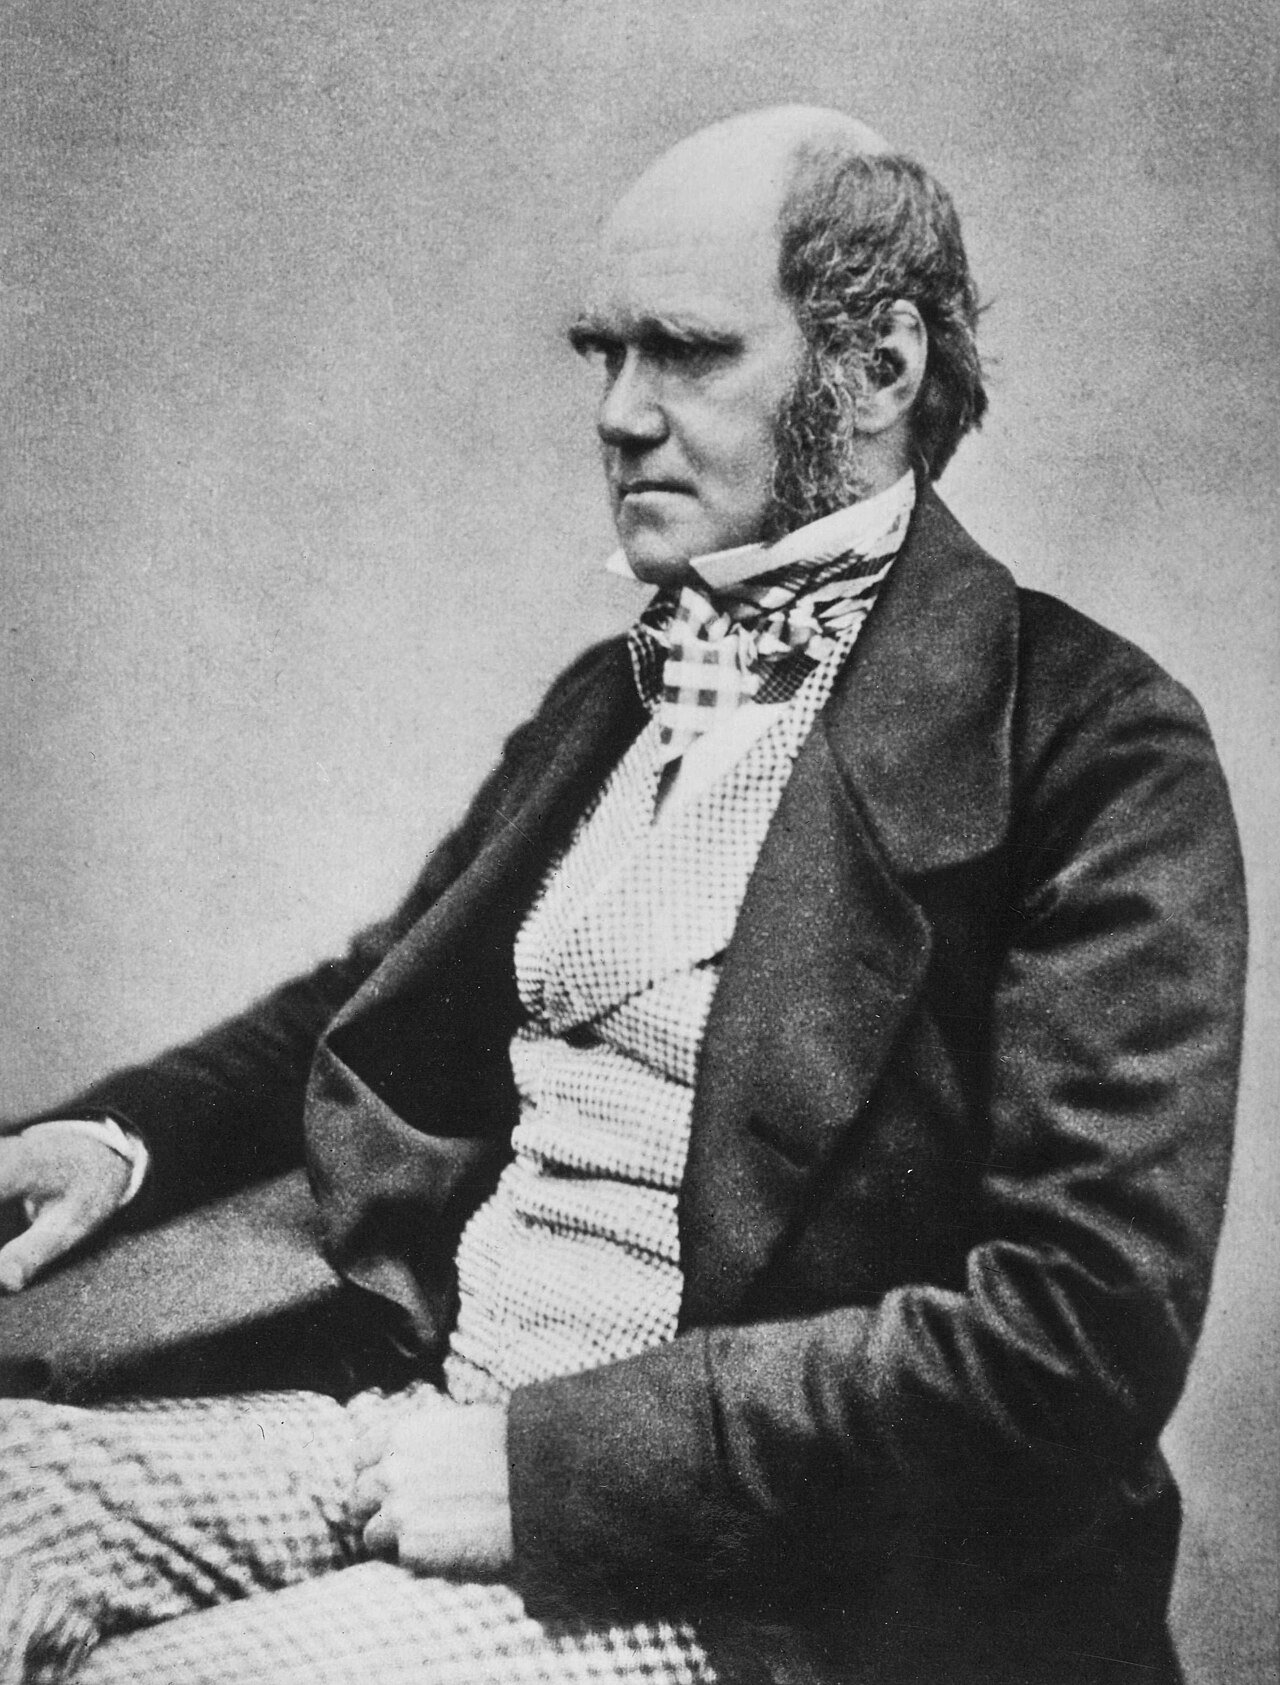
\includegraphics[width=0.36\linewidth]{images/book1/darwin.jpg}

{\small Charles Darwin, die de verwantschap van \omterm{def:g10:biodiversity-scales:species}{soorten} als eerste als een
boom tekende en het mechanisme voorstelde, de \omterm{def:g12:selection-drift-speciation:selection}{natuurlijke selectie}, dat
haar laat groeien. Foto Henry Maull en John Fox, ca.~1854, publiek
domein.}
\end{omfigure}

\begin{remark}[Wat een boom niet is]\label{rem:g12:phylogenetic-trees:not}
Een boom is een hypothese over de geschiedenis, gebouwd uit hedendaagse
\omterm{def:g10:biodiversity-scales:species}{soorten} en getoetst door elk nieuw kenmerk en elke nieuwe volgorde; zij
wordt opnieuw getekend zodra die het oneens zijn, en dat opnieuw tekenen
is het werk van het vakgebied. Zij heeft geen top en geen richting van
vooruitgang: de mens zit op één top tussen miljoenen, niet hoger en niet
meer voltooid dan de prik op een andere. En zij heeft op geen enkele top
een voorouder: de voorouders zijn de knopen, verdwenen \omterm{def:g12:selection-drift-speciation:population}{populaties} waarvan
de boom het bestaan afleidt en waarvan de fossielen, als zij worden
gevonden, náást de takken liggen en niet erop.
\end{remark}

\section{Oefeningen}

\begin{exercise}[$\star$]\label{exo:g12:phylogenetic-trees:1}
Waar staan de toppen, de knopen en de wortel van een \omterm{def:g12:phylogenetic-trees:tree}{fylogenetische boom}
voor?
\end{exercise}

\begin{exercise}[$\star$]\label{exo:g12:phylogenetic-trees:2}
Welke \omterm{def:g10:biodiversity-scales:species}{soort} is in boom A van de eerste figuur de naaste verwant van de
hagedis? En van de kikker?
\end{exercise}

\begin{exercise}[$\star$]\label{exo:g12:phylogenetic-trees:3}
Definieer een gedeelde afgeleide toestand en leg uit waarom een gedeelde
voorouderlijke toestand niet op verwantschap wijst.
\end{exercise}

\begin{exercise}[$\star$]\label{exo:g12:phylogenetic-trees:4}
Wat is een \omterm{prop:g12:phylogenetic-trees:rules}{clade}? Zijn "vogels" een \omterm{prop:g12:phylogenetic-trees:rules}{clade}? En "reptielen" (in de
dagelijkse betekenis)?
\end{exercise}

\begin{exercise}[$\star$]\label{exo:g12:phylogenetic-trees:5}
Wie is volgens de primatenboom de naaste verwant van de mens, en welke
knoop is de oudste?
\end{exercise}

\begin{exercise}[$\star\star$]\label{exo:g12:phylogenetic-trees:6}
Teken boom A van de eerste figuur opnieuw met de mens bovenaan en de
kikker onderaan, en ga na dat elke verwantschap onveranderd blijft.
\end{exercise}

\begin{exercise}[$\star\star$]\label{exo:g12:phylogenetic-trees:7}
Voeg de duif (kaken 1, ledematen 1, amnion 1, haar 0, veren 1) toe aan de
tabel van de tweede figuur en plaats haar in de boom. Wat voegt het
kenmerk "veren" toe?
\end{exercise}

\begin{exercise}[$\star\star$]\label{exo:g12:phylogenetic-trees:8}
Een dolfijn heeft een gestroomlijnd lichaam en vinnen als een haai, en
haar, melk en een zoogdierkaak. Welke boom is het spaarzaamst, en wat zijn
de vinnen?
\end{exercise}

\begin{exercise}[$\star\star$]\label{exo:g12:phylogenetic-trees:9}
Dateer met de klokfiguur de gemeenschappelijke voorouder van twee \omterm{def:g10:biodiversity-scales:species}{soorten}
waarvan het \omterm{def:g10:universal-dna:information}{DNA} 2.2\% verschilt.
\end{exercise}

\begin{exercise}[$\star\star$]\label{exo:g12:phylogenetic-trees:10}
Leg uit waarom de zin "de chimpansee is onze voorouder" de boom verkeerd
leest, en schrijf de juiste zin op.
\end{exercise}

\begin{exercise}[$\star\star$]\label{exo:g12:phylogenetic-trees:11}
Waarom wordt de prik in de tweede figuur als buitengroep gebruikt, en wat
zou er misgaan als de muis werd gebruikt?
\end{exercise}

\begin{exercise}[$\star\star\star$]\label{exo:g12:phylogenetic-trees:12}
Twee \omterm{def:g10:universal-dna:gene}{genen} geven verschillende bomen voor drie nauw verwante \omterm{def:g10:biodiversity-scales:species}{soorten} die
binnen een miljoen jaar van elkaar zijn gescheiden. Leg uit hoe dat kan
gebeuren zonder dat een van beide bomen "fout" is, met het schudden van
\omterm{def:g10:universal-dna:gene}{allelen} in de voorouderlijke \omterm{def:g12:selection-drift-speciation:population}{populatie}.
\end{exercise}

\begin{exercise}[$\star\star\star$]\label{exo:g12:phylogenetic-trees:13}
De moleculaire klok van een snel evoluerend virus loopt op 1\% per jaar;
die van een zoogdiergen op 0.3\% per miljoen jaar. Leg uit waarom de
eerste wordt gebruikt om een epidemie te volgen en de tweede om de
oorsprong van de zoogdieren te dateren, en waarom geen van beide het werk
van de ander kan doen.
\end{exercise}

\begin{exercise}[$\star\star\star$]\label{exo:g12:phylogenetic-trees:14}
Er wordt in gesteente van 150 miljoen jaar oud een fossiele vogel met
tanden en een lange benige staart gevonden. Leg uit waarom hij naast een
tak van de boom wordt geplaatst en niet op een knoop, en wat hij over die
knoop zegt.
\end{exercise}

\begin{exercise}[$\star\star\star$]\label{exo:g12:phylogenetic-trees:15}
"De boom van het leven heeft de mens aan de top." Bespreek dit in een
alinea met de leesregels, de gelijke ouderdom van de toppen, en het aantal
toppen.
\end{exercise}

\section{Probleem: Zes soorten en een klok}

\begin{problem}[{Weekendprobleem --- een boom twee keer gebouwd, uit een
kenmerkentabel en uit DNA-afstanden, de twee vergeleken, en de knopen
gedateerd}]
\label{pb:g12:phylogenetic-trees:1}
Zes \omterm{def:g10:biodiversity-scales:species}{soorten}: haai, zalm, salamander, krokodil, duif, kat. De buitengroep
is de prik. Kenmerkentabel (1 = afgeleid):

\begin{center}
\small
\begin{tabular}{lcccccc}
 & benig skelet & vier ledematen & amnionei & veren & haar & schedelopening \\ \hline
haai & 0 & 0 & 0 & 0 & 0 & 0 \\
zalm & 1 & 0 & 0 & 0 & 0 & 0 \\
salamander & 1 & 1 & 0 & 0 & 0 & 0 \\
krokodil & 1 & 1 & 1 & 0 & 0 & 0 \\
duif & 1 & 1 & 1 & 1 & 0 & 0 \\
kat & 1 & 1 & 1 & 0 & 1 & 1 \\
\end{tabular}
\end{center}

Verschillen in \omterm{def:g10:universal-dna:information}{DNA} (\%) voor één \omterm{def:g10:universal-dna:gene}{gen}:

\begin{center}
\begin{tabular}{lccccc}
 & zalm & salamander & krokodil & duif & kat \\ \hline
haai & 30 & 31 & 30 & 31 & 30 \\
zalm & & 24 & 25 & 25 & 24 \\
salamander & & & 19 & 20 & 19 \\
krokodil & & & & 8 & 15 \\
duif & & & & & 15 \\
\end{tabular}
\end{center}

\medskip
\noindent\textbf{Deel I --- Uit de kenmerken.}
\begin{enumerate}
  \item Welke afgeleide toestand wordt door de meeste \omterm{def:g10:biodiversity-scales:species}{soorten} gedeeld?
        Noem de \omterm{prop:g12:phylogenetic-trees:rules}{clade} die zij bepaalt en de \omterm{def:g10:biodiversity-scales:species}{soorten} die erbuiten blijven.
        (Het laatste kenmerk is de enkele opening in de zijkant van de
        schedel die zoogdieren hebben.)
  \item Ga verder met de volgende toestanden die het breedst worden
        gedeeld en noem de in elkaar geschoven \omterm{prop:g12:phylogenetic-trees:rules}{clades}.
  \item Veren, haar en de schedelopening komen elk bij één \omterm{def:g10:biodiversity-scales:species}{soort} voor.
        Helpen zij bij het bouwen van deze boom? Wat zou hen nuttig maken?
  \item Teken de boom, en schrijf elk kenmerk op de tak waar het
        verscheen.
  \item Wie is volgens deze tabel de naaste verwant van de krokodil?
        Welk paar valt met de tabel alleen niet te ontwarren?
\end{enumerate}

\medskip
\noindent\textbf{Deel II --- Uit het \omterm{def:g10:universal-dna:information}{DNA}.}
\begin{enumerate}[resume]
  \item Welk paar \omterm{def:g10:biodiversity-scales:species}{soorten} heeft de kleinste afstand? Voeg die als eerste
        samen.
  \item Welke \omterm{def:g10:biodiversity-scales:species}{soort} sluit zich daarna bij dat paar aan? Ga door tot de
        boom compleet is.
  \item Vergelijk de DNA-boom met de kenmerkenboom: waar zijn zij het
        eens, en wat beslist het \omterm{def:g10:universal-dna:information}{DNA} dat de kenmerken niet konden
        beslissen?
  \item De afstanden van de haai tot alle andere zijn vrijwel gelijk. Leg
        uit waarom, vanuit de vorm van de boom.
  \item De afstand krokodil--duif (8) is kleiner dan de afstand
        krokodil--kat (15). Wat zegt dat over de dagelijkse groep
        "reptielen"?
\end{enumerate}

\medskip
\noindent\textbf{Deel III --- De klok.}
Fossielen dateren de scheiding van de salamanderlijn van de amnioten op
340 miljoen jaar.
\begin{enumerate}[resume]
  \item Bereken met de afstanden salamander--amniot (ongeveer 19\%) het
        tempo van de klok in procent per miljoen jaar. (Beide lijnen zijn
        veranderd: de afstand telt de veranderingen op beide takken.)
  \item Dateer de knoop krokodil--duif en de amniotenknoop (krokodil/duif
        tegenover kat).
  \item Dateer de zalmknoop en de haaiknoop.
  \item Fossielen geven ongeveer 250 miljoen jaar voor de splitsing
        krokodil--vogel en 310 voor de amniotensplitsing. Vergelijk dat
        met jouw dateringen en becommentarieer de nauwkeurigheid van een
        klok op één \omterm{def:g10:universal-dna:gene}{gen}.
  \item De afstanden van de haai (30--31\%) overtreffen die van de zalm
        (24--25\%) nauwelijks, hoewel de haaiknoop veel ouder is. Stel een
        verklaring voor, en zeg wat dat betekent voor het dateren van heel
        oude knopen met dit \omterm{def:g10:universal-dna:gene}{gen}.
\end{enumerate}

\medskip
\noindent\textbf{Deel IV --- Lezen en benoemen.}
\begin{enumerate}[resume]
  \item Noem de \omterm{prop:g12:phylogenetic-trees:rules}{clades} van jouw boom die de kat bevatten, van de kleinste
        tot de grootste.
  \item Zijn "vissen" (haai en zalm) een \omterm{prop:g12:phylogenetic-trees:rules}{clade}? En "amnioten"?
        Verantwoord dat.
  \item Een leerling zegt dat de salamander "een tussenvorm tussen vissen
        en reptielen" is. Verbeter die uitspraak in de termen van de boom.
  \item Er wordt een fossiel met een benig skelet, vier ledematen en geen
        amnionei gevonden, gedateerd op 360 miljoen jaar. Waar zit dat ten
        opzichte van de boom, en wat bevestigt zijn datering?
  \item Geef het resultaat: de boom van de zes \omterm{def:g10:biodiversity-scales:species}{soorten} (als geneste
        haakjes), de ene verwantschap die het \omterm{def:g10:universal-dna:information}{DNA} besliste, en de
        geschatte datering van de splitsing krokodil--duif.
\end{enumerate}
\end{problem}
